\section{$* \rightarrow \omega$}

\subsection{ language operators}

We already introduced $\lim$. We can define a family of language operators, partly also derived from the study of $\Lang^\omega(reg)$. Some of these operators operate on a single language and not on the class. Let $\Lang$ be a $*$-language class. Let $L \in \Lang$.

\begin{enumerate}
\item $\ext(L) := \Set{\alpha \in \Sigma^\omega}{ \exists n \colon \alpha[0,n] \in L} = L \cdot \Sigma^\omega$
\item $\overline{\ext}(L) := \Set{\alpha \in \Sigma^\omega}{ \forall n \colon \alpha[0,n] \in L} = L \cdot \Sigma^\omega$
\item $\BC \ext$
\item $\lim(L) := \Set{ \alpha \in \Sigma^\omega }{ \forall N \colon \exists n > N \colon \alpha[0,n] \in L } = \Set{ \alpha \in \Sigma^\omega }{ \exists^\omega n \colon \alpha[0,n] \in L }$
\item $\overline{\lim}(L) := \Set{ \alpha \in \Sigma^\omega }{ \exists N \colon \forall n > N \colon \alpha[0,n] \in L }$
\item $\BC \lim$
\item Kleene-Closure of $\Lang$: $\Set{ \bigcup_{i=1}^n U_i \cdot V_i^\omega}{U_i, V_i \in \Lang}$
\item $\Set{\bigcup_{i=1}^n U_i \cdot \lim V_i}{U_i, V_i \in \K}$
\end{enumerate}

From language operators, we get language class operators in a canonical way, e.g. $\lim(\Lang) := \Set{\lim L}{L \in \Lang}$.

\subsection{$\Lang^*(reg)$}

Considering $\Lang^*(reg)$, we get a language diagram like:

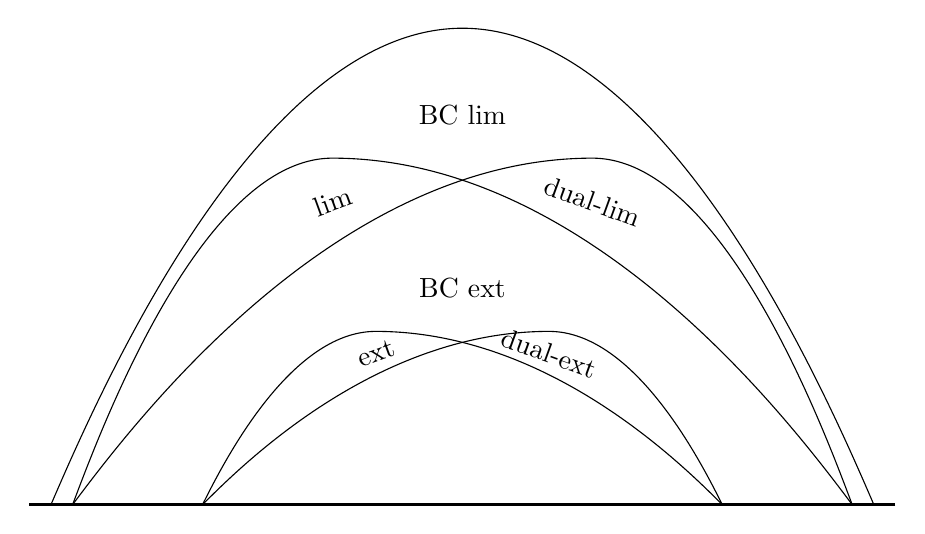
\begin{tikzpicture}
\pgftransformscale{.55}

% http://www.texample.net/tikz/examples/complexity-classes/

%%% HELP LINES - uncomment to design/extend
% \draw[step=1cm,gray,very thin] (-10,0) grid (10,12);
% \node at (0,0) {\textbf{(0,0)}};

%% Horizontal bar
\draw[very thick] (10,0) -- (-10,0);

% BC lim
\draw (-9.5,0) parabola bend (0,11) (9.5,0);
\node at (0,9) {BC lim};

% lim
\draw (-9,0) parabola bend (-3,8) (9,0);
\node[rotate=20] at (-3,7) {lim};

% dual-lim
\draw (-9,0) parabola bend (3,8) (9,0);
\node[rotate=-20] at (3,7) {dual-lim};

% BC ext
%\draw (-6.5,0) parabola bend (0,6) (6.5,0);
\node at (0,5) {BC ext};

% ext
\draw (-6,0) parabola bend (-2,4) (6,0);
\node[rotate=20] at (-2,3.5) {ext};

% dual-ext
\draw (-6,0) parabola bend (2,4) (6,0);
\node[rotate=-20] at (2,3.5) {dual-ext};

\end{tikzpicture}

where all inclusions are strict. In more detail:

... (S201,D203.1,D204,S402-S410,S106,S50)

\subsection{Curiosity}

This was studied in detail for $\Lang^*(reg)$. We are now studing relations of resulting $\omega$-language classes for different $*$-language classes.
